\begin{frame}[plain,standout]
    Problématique 1~: peut-on\\assurer la convergence des copies\\ en présence de pairs malintentionnés~?\\
    \vspace{2em}
    \begin{tikzpicture}
        \node[
            label=below:{\normalsize Mallory},
        ] {
\includegraphics[scale=.806]{collab/evil-cat.pdf}};
    \end{tikzpicture}
\end{frame}


\begin{frame}{Qu'est ce qu'un pair malintentionné~?}
    \begin{minipage}[c][.55\textheight][t]{\textwidth}
        \centering
        \begin{tikzpicture}
            \newcommand*\sep{1.5}
            \newcommand*\ang{80}
            % devices
            \path (0,0)
                +(\ang:\sep) node[
                    "Alice",
                    label={[shift={(-1,0)},opacity=0]right:{%
                        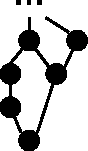
\includegraphics[scale=0.4]{collab/log-sample.pdf}%
                    }},
                    label=right:{%
                        \tikz[scale=.05]{
                            \pic {doc};
                            \pic[fill=sky] at (1,13) {square};
                            \pic[fill=olive] at (7,8) {circle};
                            \pic<2-3>[fill=pumpkin] at (7,1) {triangle};
                        }
                    },
                ](A){
\includegraphics[scale=0.35]{collab/device.pdf}}
                +(\ang-120:\sep) node[
                    "Bea" below,
                    label=right:{%
                        \tikz[scale=.05]{
                            \pic {doc};
                            \pic[fill=sky] at (1,13) {square};
                            \pic[fill=olive] at (7,8) {circle};
                            \pic<2-3>[fill=pumpkin] at (1,1) {trapeze};
                        }
                    },
                ](B){
\includegraphics[scale=0.35]{collab/device.pdf}}
                +(\ang+120:\sep) node[
                    "Mallory" below
                ](M){
\includegraphics[scale=.35]{collab/evil-cat.pdf}};
            % Links
            \draw[link] (A) -- node[midway]{\includegraphics<2>[scale=0.4]{collab/sync.pdf}} (B);
            \draw<1>[link,->] (M) -> node[pos=.33]{\tikz\pic[fill=pumpkin]{triangle};} (A);
            \draw<1>[link,->] (M) -> node[pos=.33]{\tikz\pic[fill=pumpkin]{trapeze};} (B);
            \draw<2->[link] (M) -- (A);
            \draw<2->[link] (M) -- (B);
        \end{tikzpicture}
    \end{minipage}
    \begin{minipage}{\textwidth}
        \begin{compactitemize}
            \item adversaire de la collaboration
            \begin{compactitemize}
                \item objectif~: \textbf{empêcher la convergence} des copies
                \item \emph{Byzantin}~: \textbf{pairs malintentionnés + réseau asynchrone corrompu}
            \end{compactitemize}
            \item un pair malintentionné peut compromettre la convergence par \textbf{équivoques} = modifications distinctes perçues comme identiques
        \end{compactitemize}
    \end{minipage}
\end{frame}


\begin{frame}{Journaux de modifications}
    \begin{minipage}[c][.55\textheight][t]{\textwidth}
        \centering
        \begin{tikzpicture}
            \newcommand*\sep{1.5}
            \newcommand*\ang{80}
            % devices
            \node(A) at (\ang:\sep)[
                "Alice",
                label=right:{%
                    \tikz[scale=.05]{
                        \pic<2-> {doc};
                        \pic<4->[fill=sky] at (1,13) {square};
                        \pic<5->[fill=olive] at (7,8) {circle};
                        \pic<6->[fill=pumpkin] at (7,1) {triangle};
                        %\pic<8->[fill=pumpkin] at (1,1) {trapeze};
                    }
                },
            ]{
\includegraphics[scale=0.35]{collab/device.pdf}};
            \node(B) at (\ang-120:\sep)[
                "Bea" below,
                label=right:{%
                    \tikz[scale=.05]{
                        \pic<3-> {doc};
                        \pic<5->[fill=sky] at (1,13) {square};
                        \pic<4->[fill=olive] at (7,8) {circle};
                        %\pic<8->[fill=pumpkin] at (7,1) {triangle};
                        \pic<6->[fill=pumpkin] at (1,1) {trapeze};
                    }
                },
            ]{
\includegraphics[scale=0.35]{collab/device.pdf}};
            \node(M) at (\ang+120:\sep)[
                "Mallory" below
            ]{
\includegraphics[scale=0.35]{collab/evil-cat.pdf}};
            % Logs

            \newcommand{\opDoc}{\tikz[x=1cm,y=1cm]\pic[scale=.4,fill=sky]{doc};}
            \newcommand{\opSq}{\tikz[x=1cm,y=1cm]\pic[fill=sky]{square};}
            \newcommand{\opCirc}{\tikz[x=1cm,y=1cm]\pic[fill=olive]{circle};}
            \newcommand{\opTri}{\tikz[x=1cm,y=1cm]\pic[fill=pumpkin]{triangle};}
            \newcommand{\opTra}{\tikz[x=1cm,y=1cm]\pic[fill=pumpkin]{trapeze};}

            \node[
                "\scriptsize journal de Alice",
                right=1.4 of A.north east,
                anchor=north west,
                draw,
                dashed,
                text width=5.9cm,
            ]{\begin{tikzpicture}[
                    node distance=.8cm and 1.3cm,
                    on grid
                ]
                \visible<2->{\node(new) {\opDoc};}
                \node<4->(sq)[right=of new] {\opSq};
                \node<5->(circ)[right=of sq] {\opCirc};
                \node<6->(tri)[right=of circ] {\opTri};
            \end{tikzpicture}};
            \node[
                "\scriptsize journal de Bea",
                right=1.4 of B.north east,
                anchor=north west,
                draw,
                dashed,
                text width=5.9cm,
            ]{\begin{tikzpicture}[node distance=.8cm and 1.3cm, on grid]
                \visible<3->{\node(new) {\opDoc};}
                \node<4->(circ)[right=of new] {\opCirc};
                \node<5->(sq)[right=of circ] {\opSq};
                \node<6->(tra)[right=of sq] {\opTra};
            \end{tikzpicture}};
            % Links
            \begin{scope}[every path/.style=link]
            \draw<1,3,5-> (A) -- (B);
            \draw<2>[->] (A) -> node[pos=.33]{\opDoc} (B);
            \draw<4>[->] (A) to[bend right=10] node[pos=.33]{\opSq} (B);
            \draw<4>[->] (B) to[bend right=10] node[pos=.33]{\opCirc} (A);

            \draw<1,3,6-> (A) -- (M);
            \draw<2>[->] (A) -> node[pos=.33]{\opDoc} (M);
            \draw<4>[->] (A) -> node[pos=.33]{\opSq} (M);
            \draw<5>[->] (M) -> node[pos=.33]{\opTri} (A);

            \draw<1-3,6-> (B) -- (M);
            \draw<4>[->] (B) -> node[pos=.33]{\opCirc} (M);
            \draw<5>[->] (M) -> node[pos=.33]{\opTra} (B);
            \end{scope}
        \end{tikzpicture}
    \end{minipage}
    \begin{minipage}{\textwidth}
        \begin{compactitemize}
            \item un pair enregistre dans son journal les \textbf{modifications qu'il intègre}
            \item arrangement horizontal $=$ ordre d'ajout des modifications
        \end{compactitemize}
    \end{minipage}
\end{frame}


\begin{frame}{Journaux infalsifiables}
    \begin{minipage}[c][.55\textheight][t]{\textwidth}
        \centering
        \begin{tikzpicture}
            \newcommand*\sep{1.5}
            \newcommand*\ang{80}
            % devices
            \node(A) at (\ang:\sep)[
                "Alice",
                label=right:{%
                    \tikz[scale=.05]{
                        \pic{doc};
                        \pic[fill=sky] at (1,13) {square};
                        \pic[fill=olive] at (7,8) {circle};
                        \pic[fill=pumpkin] at (7,1) {triangle};
                        \pic<4->[fill=pumpkin] at (1,1) {trapeze};
                    }
                },
            ]{
\includegraphics[scale=0.35]{collab/device.pdf}};
            \node(B) at (\ang-120:\sep)[
                "Bea" below,
                label=right:{%
                    \tikz[scale=.05]{
                        \pic{doc};
                        \pic[fill=sky] at (1,13) {square};
                        \pic[fill=olive] at (7,8) {circle};
                        \pic<4->[fill=pumpkin] at (7,1) {triangle};
                        \pic[fill=pumpkin] at (1,1) {trapeze};
                    }
                },
            ]{
\includegraphics[scale=0.35]{collab/device.pdf}};
            \node(M) at (\ang+120:\sep)[
                "Mallory" below
            ]{
\includegraphics[scale=0.35]{collab/evil-cat.pdf}};
            % Logs

            \newcommand{\opDoc}{\tikz[x=1cm,y=1cm]\pic[scale=.4,fill=sky]{doc};}
            \newcommand{\opSq}{\tikz[x=1cm,y=1cm]\pic[fill=sky]{square};}
            \newcommand{\opCirc}{\tikz[x=1cm,y=1cm]\pic[fill=olive]{circle};}
            \newcommand{\opTri}{\tikz[x=1cm,y=1cm]\pic[fill=pumpkin]{triangle};}
            \newcommand{\opTra}{\tikz[x=1cm,y=1cm]\pic[fill=pumpkin]{trapeze};}

            \node[
                "\scriptsize journal de Alice",
                right=1.4 of A.north east,
                anchor=north west,
                draw,
                dashed,
                text width=5.9cm,
                clabel/.style={font=\scriptsize,inner sep=0,anchor=south},
            ]{\begin{tikzpicture}[
                    node distance=.8cm and 1.3cm,
                    on grid
                ]
                \only<1-4>{
                    \node(a1) {\opDoc};
                    \node(a2)[right=of a1] {\opSq};
                }
                \only<1,2>{
                    \node(b1)[right=of a2] {\opCirc};
                    \node(m1)[right=of b1] {\opTri};
                }
                \only<3,4>{
                    \node(b1)[below right=of a2] {\opCirc};
                    \node(m1)[above right=of b1] {\opTri};
                }
                \only<2-4>{
                    \node[clabel] at (a1.south east) {A};
                    \node[clabel] at (a2.south east) {A};
                    \node[clabel] at (b1.south east) {B};
                    \node[clabel] at (m1.south east) {M};
                }
                \only<5>{
                    \node(a1) {$a_1$};
                    \node(a2)[right=of a1] {$a_2$};
                    \node(b1)[below right=of a2] {$b_1$};
                    \node(m1)[above right=of b1] {$m_1$};
                    \node(m1p)[below right=of m1] {$m_1'$};
                }
                \only<4>{
                    \node(m1p)[below right=of m1] {\opTra};
                    \node[clabel] at (m1p.south east) {M};
                }
                \only<3>{
                    \graph[edges={solid}]{
                        (a1) -> {
                            (a2) -> (m1),
                            (b1)
                        }
                    };
                }
                \only<4->{
                    \graph[edges={solid}]{
                        (a1) -> {
                            (a2) -> (m1),
                            (b1) -> (m1p)
                        }
                    };
                }
            \end{tikzpicture}};
            \node[
                "\scriptsize journal de Bea",
                right=1.4 of B.north east,
                anchor=north west,
                draw,
                dashed,
                text width=5.9cm,
                clabel/.style={font=\scriptsize,inner sep=0,anchor=south},
            ]{\begin{tikzpicture}[node distance=.8cm and 1.3cm, on grid]
                \only<1-4>{
                    \node(a1) {\opDoc};
                    \node(b1)[right=of a1] {\opCirc};
                }
                \only<1,2>{
                    \node(a2)[right=of b1] {\opSq};
                    \node(m1p)[right=of a2] {\opTra};
                }
                \only<3,4>{
                    \node(a2)[below right=of b1] {\opSq};
                    \node(m1p)[above right=of a2] {\opTra};
                }
                \only<2-4>{
                    \node[clabel] at (a1.south east) {A};
                    \node[clabel] at (a2.south east) {A};
                    \node[clabel] at (b1.south east) {B};
                    \node[clabel] at (m1p.south east) {M};
                }
                \only<5>{
                    \node(a1) {$a_1$};
                    \node(b1)[right=of a1] {$b_1$};
                    \node(a2)[below right=of b1] {$a_2$};
                    \node(m1p)[above right=of a2] {$m_1'$};
                    \node(m1)[below right=of m1p] {$m_1$};
                }
                \only<4>{
                    \node(m1)[below right=of m1p] {\opTri};
                    \node[clabel] at (m1.south east) {M};
                }
                \only<3>{
                    \graph[edges={solid}]{
                        (a1) -> {
                            (b1) -> (m1p),
                            (a2)
                        }
                    };
                }
                \only<4->{
                    \graph[edges={solid}]{
                        (a1) -> {
                            (a2) -> (m1),
                            (b1) -> (m1p)
                        }
                    };
                }
            \end{tikzpicture}};
            % Links
            \graph[edges={link}]{(A) -- (B) -- (M), (A) -- (M)};
            \path<3> (A) -- node[midway]{
\includegraphics[scale=0.4]{collab/sync.pdf}} (B);
        \end{tikzpicture}
    \end{minipage}
    \begin{minipage}{\textwidth}
        \begin{compactitemize}
            \item \textbf{modifications signées} par leur auteur·ice
            \item \textbf{déclaration infalsifiable des dépendances} à l'aide de \textbf{\textit{hashes}}
            \begin{compactitemize}
                \item un pair malintentionné peut déclarer des dépendances arbitraires
            \end{compactitemize}
            \item journaux avec \textbf{mêmes modifications} $\implies$ \textbf{copies convergentes}
        \end{compactitemize}
    \end{minipage}
\end{frame}


\begin{frame}{Surcoût des journaux}
    \begin{minipage}[c][.6\textheight][t]{\textwidth}
        \centering
        \begin{tikzpicture}
            \newcommand*\sep{1.5}
            \newcommand*\ang{80}
            % devices
            \node(A) at (\ang:\sep)[
                "Alice",
                label=right:{%
                    \tikz[scale=.05]{
                        \pic {doc};
                        \pic[fill=sky] at (1,13) {square};
                        \pic[fill=olive] at (7,8) {circle};
                        \pic[fill=pumpkin] at (7,1) {triangle};
                        \pic[fill=pumpkin] at (1,1) {trapeze};
                    }
                },
                label={[shift={(1,0)}]right:{%
                    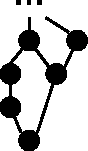
\includegraphics[scale=0.4]{collab/log-sample.pdf}%
                }},
            ]{
\includegraphics[scale=0.35]{collab/device.pdf}};
            \node(B) at (\ang-120:\sep)[
                "Bea" below,
                label=right:{%
                    \tikz[scale=.05]{
                        \pic {doc};
                        \pic[fill=sky] at (1,13) {square};
                        \pic[fill=olive] at (7,8) {circle};
                        \pic[fill=pumpkin] at (7,1) {triangle};
                        \pic[fill=pumpkin] at (1,1) {trapeze};
                    }
                },
                label={[shift={(1,0)}]right:{%
                    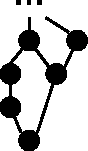
\includegraphics[scale=0.4]{collab/log-sample.pdf}%
                }},
            ](B){
\includegraphics[scale=0.35]{collab/device.pdf}};
            \coordinate(Cp) at (\ang+60:\sep*3);
            \node(C) at (Cp |- A)[
                "Carol" below,
                label=left:{%
                    \only<3>{
                        \tikz[scale=.05]{
                            \pic {doc};
                            \pic[fill=sky] at (1,13) {square};
                            \pic[fill=olive] at (7,8) {circle};
                            \pic[fill=pumpkin] at (7,1) {triangle};
                            \pic[fill=pumpkin] at (1,1) {trapeze};
                        }
                    }
                },
                label={[shift={(-1,0)},visible on=<2->]left:{%
                    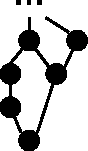
\includegraphics[scale=0.4]{collab/log-sample.pdf}%
                }},
            ]{
\includegraphics[scale=0.35]{collab/device.pdf}};
            % Links
            \draw[link] (A) -- (B);
            \draw<1>[link,->] (B) -> node[midway]{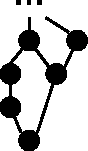
\includegraphics[scale=0.3]{collab/log-sample.pdf}} (C);
            \draw<2->[link] (B) -- (C);
        \end{tikzpicture}
    \end{minipage}
    \begin{minipage}{\textwidth}
        \begin{description}
            \item[mémoire~:] les pairs conservent leur journal
            \item[communication~:] un nouveau pair récupère un journal
            \item[calcul~:] un nouveau pair intègre chaque modification
        \end{description}
        % Passage à l'échelle
        % Confidentialité
    \end{minipage}
\end{frame}


\begin{frame}{Que font les applications de collaboration~?}
    \begin{minipage}[c][.55\textheight][t]{\textwidth}
        \centering
        \begin{tikzpicture}
            \newcommand*\sep{1.5}
            \newcommand*\ang{80}
            % devices
            \node(A) at (\ang:\sep)[
                    "Alice",
                    label=right:{%
                        \tikz[scale=.05]{
                            \pic {doc};
                            \pic[fill=sky] at (1,13) {square};
                            \pic[fill=olive] at (7,8) {circle};
                            \pic[fill=pumpkin] at (7,1) {triangle};
                            \pic[fill=pumpkin] at (1,1) {trapeze};
                        }
                    },
                    label={[shift={(1,0)}]right:{%
                        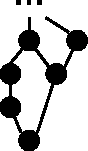
\includegraphics[scale=0.4]{collab/log-sample.pdf}%
                    }},
                ]{
\includegraphics[scale=0.35]{collab/device.pdf}};
                \node(B) at (\ang-120:\sep)[
                    "Bea" below,
                    label=right:{%
                        \tikz[scale=.05]{
                            \pic {doc};
                            \pic[fill=sky] at (1,13) {square};
                            \pic[fill=olive] at (7,8) {circle};
                            \pic[fill=pumpkin] at (7,1) {triangle};
                            \pic[fill=pumpkin] at (1,1) {trapeze};
                        }
                    },
                    label={[shift={(1,0)},visible on=<1>]right:{%
                        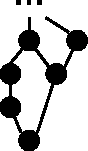
\includegraphics[scale=0.4]{collab/log-sample.pdf}%
                    }},
                    label={[shift={(1,0)}, visible on=<2->]right:{%
                        
\includegraphics[scale=0.4]{collab/pruned-log.pdf}%
                    }},
                ]{
\includegraphics[scale=0.35]{collab/device.pdf}};
                \coordinate(Cp) at (\ang+60:\sep*3);
                \node(C) at (Cp |- A)[
                    "Carol",
                    label={[visible on=<4>]left:{%
                        \tikz[scale=.05]{
                            \pic {doc};
                            \pic[fill=sky] at (1,13) {square};
                            \pic[fill=olive] at (7,8) {circle};
                            \pic[fill=pumpkin] at (7,1) {triangle};
                            \pic[fill=pumpkin] at (1,1) {trapeze};
                        }
                    }},
                ]{
\includegraphics[scale=0.35]{collab/device.pdf}};
            % Links
            \draw[link] (A) -- (B);
            \draw<3>[link,->] (B) -> node[midway]{
                \tikz[scale=.05]{
                    \pic {doc};
                    \pic[fill=sky] at (1,13) {square};
                    \pic[fill=olive] at (7,8) {circle};
                    \pic[fill=pumpkin] at (7,1) {triangle};
                    \pic[fill=pumpkin] at (1,1) {trapeze};
                }
            } (C);
            \draw<4>[link] (B) -- (C);
        \end{tikzpicture}
    \end{minipage}
    \begin{minipage}{\textwidth}
        \begin{compactitemize}
            \item hypothèse~: taille contenu $<$ taille journal
            \item \textbf{troncature} du journal \textbf{sans coordination}
            \item \textbf{transmission de l'état de la copie} aux nouveaux pairs
        \end{compactitemize}
    \end{minipage}
\end{frame}


\begin{frame}{Diffucltés en présence de pairs malintentionnés}
    \begin{minipage}[c][.55\textheight][t]{\textwidth}
        \centering
        \begin{tikzpicture}
            \newcommand*\sep{1.5}
            \newcommand*\ang{80}
            % devices
            \node(A) at (\ang:\sep)[
                    "Alice",
                ]{
\includegraphics[scale=0.35]{collab/device.pdf}};
            \node(B) at (\ang-120:\sep)[
                "Bea" below,
            ]{
\includegraphics[scale=0.35]{collab/device.pdf}};
            \coordinate(Cp) at (\ang+60:\sep*3);
            \node(C) at (Cp |- A)[
                "Carol",
            ]{
\includegraphics[scale=0.35]{collab/device.pdf}};
            \node(M) at (\ang+120:\sep)[
                "Mallory" below
            ]{
\includegraphics[scale=0.35]{collab/evil-cat.pdf}};
            % Links
            \draw[link] (A) -- node[midway]{\includegraphics<1>[scale=0.4]{collab/sync.pdf}} (B) -- (M) -- (A);
            \draw<3>[link,->] (M) -> node[midway]{
                \tikz[scale=.05]{
                    \pic {doc};
                    \pic[fill=pumpkin] at (7,1) {triangle};
                }
            } (C);
            \draw<4->[link] (M) -- (C);
            \draw<4,5>[link] (A) -- node[midway]{\includegraphics<4>[scale=0.4]{collab/sync.pdf}} (C);
            % docs
            \node also[
                label=right:{%
                    \tikz[scale=.05]{
                        \pic {doc};
                        \pic[fill=sky] at (1,13) {square};
                        \pic[fill=olive] at (7,8) {circle};
                        \pic[fill=pumpkin] at (7,1) {triangle};
                        %\pic[fill=pumpkin] at (1,1) {trapeze};
                    }
                },
                label={[shift={(1,0)}]right:{%
                    
\includegraphics[scale=0.4]{collab/pruned-log.pdf}%
                }},
            ](A);
            \node also[
                label=right:{%
                    \tikz[scale=.05]{
                        \pic {doc};
                        \pic[fill=sky] at (1,13) {square};
                        \pic[fill=olive] at (7,8) {circle};
                        %\pic[fill=pumpkin] at (7,1) {triangle};
                        \pic[fill=pumpkin] at (1,1) {trapeze};
                    }
                },
                label={[shift={(1,0)}]right:{%
                    
\includegraphics[scale=0.4]{collab/pruned-log.pdf}%
                }},
            ](B);
            \node also[
                label={[visible on=<4->]left:{%
                    \tikz[scale=.05]{
                        \pic {doc};
                        \pic[fill=pumpkin] at (7,1) {triangle};
                    }
                }},
            ](C);
        \end{tikzpicture}
    \end{minipage}
    \begin{minipage}{\textwidth}
        \begin{compactitemize}
            \item le journal \textbf{ne peut pas être tronqué arbitrairement}
            \begin{compactitemize}
                \item la détection d'équivoque pourrait être compromise
            \end{compactitemize}
            \item un pair malintentionné peut transmettre un \textbf{état falsifié}
        \end{compactitemize}
    \end{minipage}
\end{frame}


\begin{frame}{Notre approche}
    \begin{minipage}[c][.55\textheight][t]{\textwidth}
        \centering
        \begin{tikzpicture}[x radius=2cm]
            \newcommand*\sep{1.5}
            \newcommand*\ang{80}
            % devices
            \node(A) at (\ang:\sep)[
                "Alice",
            ]{
\includegraphics[scale=0.35]{collab/device.pdf}};
            \node(B) at (\ang-120:\sep)[
                "Bea" below,
            ]{
\includegraphics[scale=0.35]{collab/device.pdf}};
            \coordinate(Cp) at (\ang+60:\sep*3);
            \node(C) at (Cp |- A)[
                "Carol" below,
            ]{
\includegraphics[scale=0.35]{collab/device.pdf}};
            % Links
            \draw[link] (A) -- (B);
            \draw<1>[link, ->] (B) ->%
                    node[midway,above]{
\includegraphics[scale=0.3]{collab/pruned-log.pdf}}%
                    node[midway,below]{
                        \tikz[scale=.05]{
                            \pic {doc};
                            \pic[fill=sky] at (1,13) {square};
                            \pic[fill=olive] at (7,8) {circle};
                            \pic[fill=pumpkin] at (7,1) {triangle};
                            \pic[fill=pumpkin] at (1,1) {trapeze};
                        }
                    }%
                (C);
            \draw<2->[link] (B) -- (C);
            % docs
            \node also[
                label=right:{%
                    \tikz[scale=.05]{
                        \pic {doc};
                        \pic[fill=sky] at (1,13) {square};
                        \pic[fill=olive] at (7,8) {circle};
                        \pic[fill=pumpkin] at (7,1) {triangle};
                        \pic[fill=pumpkin] at (1,1) {trapeze};
                    }
                },
                label={[shift={(1,0)}]right:{%
                    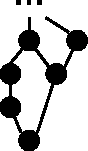
\includegraphics[scale=0.4]{collab/log-sample.pdf}%
                }},
            ](A);
            \node also[
                label=right:{%
                    \tikz[scale=.05]{
                        \pic {doc};
                        \pic[fill=sky] at (1,13) {square};
                        \pic[fill=olive] at (7,8) {circle};
                        \pic[fill=pumpkin] at (7,1) {triangle};
                        \pic[fill=pumpkin] at (1,1) {trapeze};
                    }
                },
                label={[shift={(1,0)}]right:{%
                    
\includegraphics[scale=0.4]{collab/pruned-log.pdf}%
                }},
            ](B);
            \node also[
                label={[visible on=<2->]left:{%
                    \tikz[scale=.05]{
                        \pic {doc};
                        \pic[fill=sky] at (1,13) {square};
                        \pic[fill=olive] at (7,8) {circle};
                        \pic[fill=pumpkin] at (7,1) {triangle};
                        \pic[fill=pumpkin] at (1,1) {trapeze};
                    }
                }},
                label={[shift={(-1,0)},visible on=<2->]left:{%
                    
\includegraphics[scale=0.4]{collab/pruned-log.pdf}%
                }},
            ](C);
        \end{tikzpicture}
    \end{minipage}
    \begin{minipage}{\textwidth}
        \begin{compactitemize}
            \item \textbf{troncature sans coordination} reposant sur le concept de \textbf{stabilité}
            \begin{compactitemize}
                \item conservation de modifications pour la détection d'équivoques
            \end{compactitemize}
            \item transmission d'un \textbf{état authentifiable} et journal tronqué
            \begin{compactenumerate}
                \item vérifie la cohérence du journal tronqué
                \item authentifie le contenu à partir du journal
            \end{compactenumerate}
        \end{compactitemize}
    \end{minipage}
\end{frame}


\begin{frame}{Journal causal}
    \begin{minipage}[c][.48\textheight][t]{\textwidth}
        \begin{tikzpicture}[x=1.3cm,y=.8cm,every node/.style={compact}]
            \node at (0,.9) {};
            \begin{scope}
                \node(A)["Alice" username] at (-1,0) {
                    
\includegraphics[scale=.35]{collab/device.pdf}
                };
                \node(a1)[
                    fillhighlight on=<{1,7}>,
                ] at (0,0) {$a_1$};
                \node(a2)[
                    disabled on={<1>},
                    fillhighlight on=<{2,7}>,
                ] at (1,0) {$a_2$};
                \node(b1)[
                    disabled on=<1-2>,
                    fillhighlight on=<8>,
                ] at (2,-1) {$b_1$};
                \node[
                    disabled on=<1-2>,
                    fillhighlight on=<{3,7}>,
                ] (a3) at (3,0) {$a_3$};
                \graph{
                    (a1) ->[disabled on=<1>] (a2),
                    (a1) ->[disabled on=<1-2>] (b1),
                    {(a2), (b1)} ->[disabled on=<1-2>] (a3)
                };
            \end{scope}
            \begin{scope}[shift={(0,-2cm)}]
                \node(B)["Bea" username] at (-1,0) {
                    
\includegraphics[scale=.35]{collab/device.pdf}
                };
                \node(a1)[
                    fillhighlight on=<7>,
                ] at (0,0) {$a_1$};
                \node(b1)[
                    fillhighlight on=<{4,8}>,
                ] at (1,0) {$b_1$};
                \node(a2)[
                    disabled on=<4>,
                    fillhighlight on=<6-7>,
                ] at (2,-1) {$a_2$};
                \node[
                    disabled on=<4>,
                    fillhighlight on=<6-7>,
                ] (a3) at (3,0) {$a_3$};
                \node(b2)[
                    disabled on=<4>,
                    fillhighlight on=<{5-6,8}>,
                ] at (4,0) {$b_2$};
                \graph[edges={disabled on=<4>}]{
                    (a1) -> {
                        (a2),
                        (b1)
                    },
                    (b1) ->[visible on=<{1-5,7-}>] (a3) ->[visible on=<{1-5,7-}>] (b2),
                    (a2) -> (a3)
                };
                \draw<6>[->] (b1) to[bend left=15] (b2);
                \node<6> at (b2.east)[anchor=west]{\color{invalid} \xmark};
            \end{scope}
        \end{tikzpicture}
    \end{minipage}
    \begin{minipage}{\textwidth}
        \textbf{Invariants}
        \begin{compactenumerate}
            \item {\only<7->{\transparent{.6}}une modification du possesseur du journal dépend des précédentes}
            \item {\only<-6>{\transparent{.6}}ordre linéaire des modification de chaque pair}
        \end{compactenumerate}
        % \begin{compactitemize}
        %     \item le possesseur du journal observe toutes les modifications
        %     \item les dépendances traduisent les observations des autres pairs
        % \end{compactitemize}
    \end{minipage}
\end{frame}


\begin{frame}{Stabilité causale}
    \begin{minipage}[c][.48\textheight][t]{\textwidth}
        \begin{tikzpicture}[x=1.3cm,y=.8cm,every node/.style={compact}]
            \node at (0,.9) {};
            \begin{scope}
                \node["Alice" username] at (-1,0) {
                    
\includegraphics[scale=0.35]{collab/device.pdf}
                };
                \node(a1)[
                    stable on=<2->,
                ] at (0,0) {$a_1$};
                \node(a2)[
                    stable on=<5->,
                ] at (1,0) {$a_2$};
                \node(b1)[
                    fillhighlight on=<1>,
                    stable on=<2->,
                ] at (2,-1) {$b_1$};
                \node(a3)[
                    stable on=<5->,
                ] at (3,0) {$a_3$};
                \graph{
                    (a1) -> {(a2), (b1)} -> (a3)
                };
                \only<1>{
                    \node(b2) at (4,0) {$b_2$};
                    \graph[edges={dashed}]{
                        (a3) ->["?"] (b2),
                        (b1) ->["?" below] (b2)
                    };
                }
                \only<5>{
                    \node(b2)[
                        stable,
                    ] at (4,0) {$b_2$};
                    \graph{
                        (a3) -> (b2)
                    };
                }
            \end{scope}
            \begin{scope}[shift={(0,-2cm)}]
                \node at (0,.9) {};
                \node["Bea" {below,username}, "x" {opacity=0,username}] at (-1,0) {
                    
\includegraphics[scale=0.35]{collab/device.pdf}
                };
                \node(a1)[
                    stable on=<4->,
                ] at (0,0) {$a_1$};
                \node(b1)[
                    stable on=<4->,
                ] at (1,0) {$b_1$};
                \node(a2)[
                    stable on=<4->,
                ] at (2,-1) {$a_2$};
                \node(a3)[
                    fillhighlight on=<3>,
                    stable on=<4->,
                ] at (3,0) {$a_3$};
                \node(b2) at (4,0) {$b_2$};
                \graph{
                    (a1) -> {(a2), (b1)} -> (a3) -> (b2)
                };
            \end{scope}
        \end{tikzpicture}
    \end{minipage}
    \begin{minipage}{\textwidth}
        \begin{definition}
            modification stable $\iff$ dépendance de toute modification \textbf{ultérieurement acceptée} dans le journal.
        \end{definition}
        \begin{theorem}
            modification stable $\iff$ observée par chaque pair au sein du journal.
        \end{theorem}
    \end{minipage}
\end{frame}


\begin{frame}{Jounal \acf{VFJC}}
    \begin{minipage}[c][.3\textheight][t]{\textwidth}
        \begin{tikzpicture}[x=1.3cm,y=.8cm,every node/.style={compact}]
            \node at (0,.9) {};
            \node(A)["Alice" username] at (-1,0) {
                
\includegraphics[scale=0.35]{collab/device.pdf}
            };
            \node(a1) at (0,0) {$a_1$};
            \node(m1)[
                fillhighlight on=<1>,
                disabled on=<3>,
            ] at (1,0) {$m_1$};
            \node(b1)at (2,-1) {$b_1$};
            \node(a2)[disabled on=<3>]  at (3,0) {$a_2$};
            \node(m1p)[
                fillhighlight on=<{1,5}>,
                disabled on=<2>,
            ] at (4,-1) {$m_1'$};
            \node(b2)[
                disabled on=<2>,
                "\color{invalid} \xmark" {right, visible on=<4>},
            ] at (5,-1) {$b_2$};
            \node(a3)[
                "$\scriptstyle\set*{M}$" {visible on=<5>},
                disabled on=<2-4>,
            ] at (6,0) {
\includegraphics[scale=.15]{collab/eye.pdf}};
            \graph{
                (a1) ->[disabled on=<3>] (m1) ->[disabled on=<3>] (a2),
                (a1) -> (b1),
                (b1) ->[disabled on=<3>] (a2),
                (b1) ->[disabled on=<2>] (m1p) ->[disabled on=<2>] (b2),
                {(a2), (b2)} ->[disabled on=<2-4>] (a3),
                (a2) ->[visible on=<4>] (b2)
            };
        \end{tikzpicture}
    \end{minipage}
    \begin{minipage}{\textwidth}
        \textbf{Invariants}
        \begin{compactenumerate}
            \item {\transparent{.6}une modification du possesseur du journal dépend des précédentes}
            \item {\transparent{.6}ordre linéaire des modification de chaque pair honnête}
            \item une modification \textbf{dépend directement} de modifications \textbf{présumées linéaires}
            \begin{compactitemize}
                \item {\only<1-4>{\transparent{.6}}une modification non-linéaire est acceptée indirectement}
                \item {\only<1-4>{\transparent{.6}}le possesseur du jorunal ne peut plus accepter directement de modifications d'un pair reconnu malintentionné}
            \end{compactitemize}
        \end{compactenumerate}
    \end{minipage}
\end{frame}


\begin{frame}{Stabilité et invariants de journaux}
    \begin{tikzpicture}[every node/.append style={
        align=center,
        inner sep=.5em,
    },node distance=.3cm and 1.6cm]
        \node(honest){environnement\\honnête};
        \node(malicious)[right=of honest]{environnement\\malintentionné};
        \node(static)[below left=of honest]{groupe\\statique};
        \node(dyn)[below=of static]{groupe\\dynamique};

        \node(causal)[below=of honest]{journal causal\footcite{hutto_1990_causal}\\stabilité causale\footcite{baquero_2018_pure-op-crdt}};
        \node(vfjc)[below=of malicious]{journal VFJC\footcite{mahajan_2011_cac}\\ \textbf{stabilité VFJC}};
        \node(dyncausal)[below=of causal]{\textbf{journal DynCausale}\\ \textbf{stabilité DynCausale}};
        \node(dynvfjc)[below=of vfjc]{\textbf{journal DynVFJC}\\ \textbf{stabilité DynVFJC}};

        \draw[thick] (dyn.west |- honest.south) -- (malicious.south -| dynvfjc.east);
        \draw[thick] (honest.north -| dyn.east) -- (dyn.south east);
    \end{tikzpicture}
    groupe statique = groupe avec un ensemble défini de pairs\\
    groupe dynamique = groupe dont la composition évolue
\end{frame}


\begin{frame}{Journal \acs{VFJC}}
    \begin{minipage}[c][.5\textheight][t]{\textwidth}
        \begin{tikzpicture}[x=1.3cm,y=.8cm,every node/.style={compact}]
            \node at (0,1.7) {};
            \node["Alice" username] at (-1,0) {
                
\includegraphics[scale=0.35]{collab/device.pdf}
            };
            \node(a1)[
                fillhighlight on=<1>,
                "\scriptsize stable~?" {below, visible on=<1>},
            ] at (0,0) {$a_1$};
            \node(m1) at(1,0) {$m_1$};
            \node(b1) at (2,-1) {$b_1$};
            \node(a2) at(3,0) {$a_2$};
            \node<2>(m1p) at (4,-2) {$m_1'$};
            \node<2>(b2) at (5,-1) {$b_2$};
            \node<3>(b1p) at (4,1) {$b_1'$};
            \node<3>(m2) at (5,1) {$m_2$};
            \node(a3) at (6,0) {
\includegraphics[scale=.15]{collab/eye.pdf}};
            \graph{
                (a1) -> (m1) -> (a2) -> (a3),
                (a1) -> (b1) -> (a2),
            };
            \only<2>{
                \graph{
                    (b1) -> (b2) -> (a3),
                    (m1p) -> (b2),
                };
            }
            \only<3>{
                \graph{
                    (m1) ->[bend left=25] (m2),
                    (b1p) -> (m2) -> (a3),
                };
            }
        \end{tikzpicture}
    \end{minipage}
    \begin{minipage}{\textwidth}
        \begin{compactitemize}
            \item le possesseur du journal \textbf{présume honnêtes} les autres pairs
            \begin{compactitemize}
                \item il s'attend à ce qu'ils soient \textbf{potentiellement malintentionnés}
            \end{compactitemize}
        \end{compactitemize}
    \end{minipage}
\end{frame}


\begin{frame}{Contribution~: Stabilité \acs{VFJC}}
    \newcommand{\eye}{
\includegraphics[scale=.15]{collab/eye.pdf}}
    \begin{minipage}[c][.3\textheight][t]{\textwidth}
        \begin{tikzpicture}[x=1.3cm,y=-.8cm,every node/.style={compact}]
            \node at (0,.9) {};
            \node["Alice" username] at (-1,0) {
                
\includegraphics[scale=0.35]{collab/device.pdf}
            };
            \node(a1)[stable] at (0,0) {$a_1$};
            \node(m1) at(1,0) {$m_1$};
            \node(a2) at(2,0) {$a_2$};
            \node(b1)[stable] at (3,1) {$b_1$};
            \node(m1p)[stable] at (4,1) {$m_1'$};
            \node(b2) at (5,1) {$b_2$};
            \node[
                "$\scriptstyle\set*{M}$"
            ] (a3) at (6,0) {\eye};
            \graph{
                (a1) -> (m1) -> (a2),
                (a1) -> (b1) -> (m1p) -> (b2),
                {(a2), (b2)} -> (a3)
            };
        \end{tikzpicture}
    \end{minipage}
    \begin{minipage}{\textwidth}
        \centering
        \begin{tabular}{cc}
            permutation & chaîne de dépendance\\
            \toprule
            $M, B, A$ & $m_1', b_2, \eye$\\
            $B, M, A$ & $b_2, \eye, \eye$\\
        \end{tabular}
    \end{minipage}
    \begin{minipage}{\textwidth}
        \begin{theorem}
            modification $x$ stable $\iff$ pour toute permutation $p_1, \dotsc, p_N$ des pairs avec $p_N$ le possesseur du journal, il existe une chaîne de dépendances $x, x_1, \dotsc, x_N$ telle que $x_i$ a pour auteur ou reconnaît malintentionné $p_i$.
        \end{theorem}
    \end{minipage}
\end{frame}


\begin{frame}{Contribution~: Jounal causal dynamique}
    \begin{minipage}[c][.3\textheight][t]{\textwidth}
        \begin{tikzpicture}[x=1.33cm,y=.8cm,every node/.style={compact}]
            \node at (0,.9) {};
            \node["Alice" username] at (-1,0) {
                
\includegraphics[scale=0.35]{collab/device.pdf}
            };
            \node(a1)[
                fillhighlight on=<3>,
                "$\scriptstyle\trm{invit}({A,B})$"{
                    fillhighlight on=<{1,3}>,
                },
            ] at (0,0) {$a_1$};
            \node(a2)[
                fillhighlight on=<3>,
            ] at (1,0) {$a_2$};
            \node(b1)[
                fillhighlight on=<1>,
                "$\scriptstyle\trm{invit}(C)$"{
                    below,
                    fillhighlight on=<2>%
                },
            ] at (2,-1) {$b_1$};
            \node(c1)[
                fillhighlight on=<2>,
            ] at (3,0) {$c_1$};
            \node(b2)[
                fillhighlight on=<1>,
            ] at (4,0) {$b_2$};
            \graph{
                (a1) -> {(a2), (b1)} -> (c1) -> (b2)
            };
        \end{tikzpicture}
    \end{minipage}
    \begin{minipage}{\textwidth}
        \begin{compactitemize}
            \item suivi de la composition du groupe via les invitations
            \item les modifications d'un pair dépendent des dépendances de son invit.
        \end{compactitemize}
        \medskip
        \textbf{Invariants}
        \begin{compactenumerate}
            \item {\transparent{.6}une modification du possesseur du journal dépend des précédentes}
            \item {\transparent{.6}ordre linéaire des modifications de chaque pair}
            \item les modifications d'un pair dépendent de son invitation
        \end{compactenumerate}
    \end{minipage}
\end{frame}


\begin{frame}{Contribution~: Stabilité causale dynamique}
    \begin{minipage}[c][.3\textheight][t]{\textwidth}
        \begin{tikzpicture}[x=1.3cm,y=.8cm,every node/.style={compact}]
            \node at (0,.9) {};
            \node["Alice" username] at (-1,0) {
                
\includegraphics[scale=0.35]{collab/device.pdf}
            };
            \node(a1)[
                stable,
                fillhighlight on=<1>,
                "$\scriptstyle\trm{invit}({A,B})$"{
                    fillhighlight on=<2->,
                },
            ] at (0,0) {$a_1$};
            \node(a2)[
                stable on=<6->,
                fillhighlight on=<{2,3,5-6}>,
            ] at (1,0) {$a_2$};
            \graph{
                (a1) -> (a2)
            };
            \only<3->{
                \node(b1)[
                    stable,
                    fillhighlight on=<4>,
                    "$\scriptstyle\trm{invit}(C)$"{
                        fillhighlight on=<{3,5-}>,
                        below,
                    },
                ] at (2,-1) {$b_1$};
                \graph{
                    (a1) -> (b1)
                };
            }
            \only<5->{
                \node(c1)[
                    stable on=<6->,
                    fillhighlight on=<5-6>,
                ] at (3,0) {$c_1$};
                \graph{
                    {(a2), (b1)} -> (c1)
                };
            }
            \only<6->{
                \node(b2)[
                    fillhighlight on=<7>,
                ] at (4,0) {$b_2$};
                \graph{
                    (c1) -> (b2)
                };
            }
        \end{tikzpicture}
    \end{minipage}
    \begin{minipage}{\textwidth}
        \begin{compactitemize}
            \item observateurs honnêtes requis =
            \begin{compactitemize}
                \item[+] pairs invités dans les dépendances
                \item[+] pairs invités en concurrence
            \end{compactitemize}
    \end{compactitemize}
    \end{minipage}
    \begin{minipage}{\textwidth}
        % \begin{tabular}{ccc}
        %     $a_2$ & $a_3, c_1, b_2$ & $b_1$ \\
        %     \toprule
        %     $\set*{A}$ & $\set*{A, B}$ & $\set*{A, B}$ \\
        %     $\emptyset$ & $\set*{C}$ & $\emptyset$ \\
        % \end{tabular}
    \end{minipage}
    \begin{minipage}{\textwidth}
        \begin{theorem}
            modification stable $\iff$ elle est observée par chacun de ses observateurs honnêtes requis au sein du journal.
        \end{theorem}
    \end{minipage}
\end{frame}


\begin{frame}{Résumé des contributions}
    \begin{compactitemize}
        \item contributions
        \begin{compactitemize}
            \item formalisation et généralisation du \textbf{concept de stabilité}
            \item formalisation des journaux et leurs invariants
            \item protocole à \textbf{journaux complets} et protocole à \textbf{journaux tronqués}
            \item formalisation et preuves des garanties offertes par les protocoles
            \item \textbf{algorithme à complexité linéaire}\singlefootnote{par rapport à la taille du journal} pour déterminer un sous-ensemble de modifications stables
        \end{compactitemize}
        \item notre approche
        \begin{compactitemize}
            \item protége la convergence avec des \textbf{journaux infalsifiables tronqués}
            \item tolère la présence de \textbf{pairs malintentionnés}
            \item est adapté aux \textbf{groupes dynamiques}
            \item \textbf{sans coordination}
        \end{compactitemize}
        \item limite~: des pairs inactifs peuvent \textbf{bloquer la troncature}
    \end{compactitemize}
\end{frame}

